\documentclass[11pt,letterpaper]{article}

% ---------- Paquetes ----------
\usepackage[utf8]{inputenc}
\usepackage[T1]{fontenc}
\usepackage[spanish,es-noshorthands]{babel}
\usepackage{lmodern}
\usepackage[margin=2.5cm]{geometry}
\usepackage{amsmath,amssymb,amsthm}
\usepackage{graphicx}
\usepackage{booktabs}
\usepackage{siunitx}
\usepackage{caption}
\usepackage[hidelinks]{hyperref}
\usepackage{listings}

\graphicspath{{figuras/}}
\decimalpoint

% ---------- Notación (usar estos comandos para que todo sea igual) ----------
\newcommand{\lat}{\varphi}
\newcommand{\lon}{\lambda}
\newcommand{\qiso}{q(\varphi)}
\newcommand{\region}{\Omega}
\newcommand{\frontera}{\partial\Omega}
\newcommand{\dist}{\delta(\Omega)}

% ---------- Datos del documento ----------
\title{Proyecciones conformes óptimas para el análisis de datos geoespaciales en México}
\author{
  Integrante 1 \quad A00000000 \\
  Integrante 2 \quad A00000000 \\
  Integrante 3 \quad A00000000 \\
  Integrante 4 \quad A00000000 \\[1em]
  Profesor(a): Nombre \\
  Materia (Grupo 602) \\
  Tecnológico de Monterrey, Campus Monterrey
}
\date{\today}

\begin{document}
\maketitle

% Responsable: Persona 4. ~150 palabras. Se escribe al final con los números de la tabla.
\begin{abstract}
\textbf{Pendiente.} Un párrafo con la respuesta para el cliente: qué proyección
usar, $\delta$ de Mercator, Lambert y la óptima, error típico en distancias y
cuánto se gana con la óptima.
\end{abstract}

% Responsable: Persona 4. ~300 palabras.
\section{Introducción y contexto del problema}

\subsection{Por qué los datos geoespaciales necesitan coordenadas planas}

La latitud $\lat$ y la longitud $\lon$ son ángulos, no distancias. Un grado de
latitud mide siempre unos 111.2~km, pero uno de longitud mide
$R\cos\lat\,\pi/180$: 111.2~km en el ecuador y 97.3~km a $29^\circ$\,N, en
Sonora. Los algoritmos del cliente (k-means, búsqueda de vecinos cercanos con
árboles k-d, interpolación espacial por IDW o kriging, mapas de calor por
densidad de núcleo y optimización de rutas) suponen distancias euclidianas.
Con millones de registros lo práctico es proyectar una sola vez a $(x, y)$ y
trabajar en el plano, en lugar de calcular la distancia sobre la esfera para
cada par. La pregunta es cuánto error mete ese paso.

\subsection{Por qué no existe un mapa perfecto}

En el siglo XVIII Euler demostró que ningún mapa plano conserva todas las
distancias de la esfera \cite{snyder1987}. La razón de fondo es el Teorema
Egregium de Gauss:
la curvatura gaussiana no cambia bajo isometrías, y la de la esfera es $1/R^2$
mientras que la del plano es 0 \cite{docarmo1976}. Toda proyección renuncia a
algo: las conformes conservan los ángulos, las equivalentes conservan las
áreas y las equidistantes conservan las distancias solo en ciertas
direcciones.

\subsection{Qué significa que una proyección sea conforme}

Una proyección es conforme si conserva los ángulos o, lo que es lo mismo, si
en cada punto estira todas las direcciones por el mismo factor $\sigma$. Eso
es lo que le importa al cliente: una distancia corta en el mapa es $\sigma$
veces la real sin importar su orientación, así que vecinos y grupos solo
dependen de cuánto varía $\sigma$ dentro del país. Hoy el cliente usa
Mercator; INEGI usa la Cónica Conforme de Lambert con paralelos estándar en
$17.5^\circ$ y $29.5^\circ$\,N, registrada como EPSG:6372 \cite{epsg} (a veces
se cita como EPSG:6361, un código que no aparece en el registro como sistema
de coordenadas). Esta wiki
compara las dos con la proyección conforme óptima para México y responde
cuál conviene, cuánto error mete cada una y cuánto se puede ganar.

\subsection{Variables del problema}

\begin{itemize}
  \item $\lat$, $\lon$: latitud y longitud (grados en el texto, radianes en las
    fórmulas); $R = 6\,371.0088$~km, el radio medio de la Tierra.
  \item $q(\lat)$: latitud isométrica, y $w = \lon + i\,q$, la coordenada
    compleja sobre la esfera (sección~\ref{sec:fundamentos}).
  \item $z = x + iy = f(w)$: coordenadas planas, en metros.
  \item $\sigma$: factor de escala, la longitud en el mapa dividida entre la
    real. En Mercator y Lambert depende solo de $\lat$; en la proyección
    óptima depende también de la forma de la región.
  \item $\region$: México continental (de $14.53^\circ$ a $32.72^\circ$\,N y de
    $86.7^\circ$ a $117.1^\circ$\,O), con frontera $\frontera$, y
    $\dist$, la distorsión de una proyección sobre $\region$ (Paso~3).
\end{itemize}

% Responsable: Persona 1. ~450 palabras.
\section{Fundamentos teóricos}

\subsection{Funciones analíticas y ecuaciones de Cauchy--Riemann}
% f = u + iv, u_x = v_y, u_y = -v_x. df = f'(z) dz. Contraejemplo z^2.

\subsection{Funciones armónicas y problema de Dirichlet}
% Conjugada armónica, ln|f'| = Re(ln f'), existencia y unicidad, principio del máximo.

\subsection{Esfera de Riemann y proyección estereográfica}

\subsection{Coordenada compleja sobre la esfera}
% Ejemplo de ecuación numerada:
\begin{equation}
  ds^2 = R^2\cos^2\lat\,|dw|^2, \qquad
  \sigma(w) = \frac{|f'(w)|}{R\cos\lat}
  \label{eq:sigma}
\end{equation}

% Figura 1 (Persona 3): retícula de México bajo dos proyecciones.
% \begin{figure}[ht]
%   \centering
%   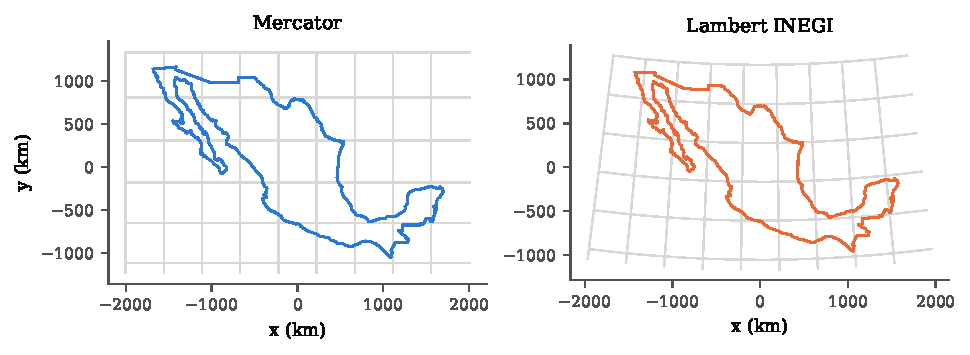
\includegraphics[width=0.9\linewidth]{fig1_reticula}
%   \caption{Retícula de meridianos y paralelos sobre México. Fuente: elaboración propia.}
%   \label{fig:reticula}
% \end{figure}

% Responsables: Pasos 1, 2 y teoría del 4: Persona 1. Paso 3: Persona 4.
% Numérico del 4: Persona 2. Paso 5: Persona 3. ~900 palabras en total.
\section{Solución del problema del cliente}

\subsection{Paso 1. Mercator}

La proyección más sencilla es tomar $f(w) = R\,w$, es decir,
\begin{equation}
  x = R\,\lon, \qquad y = R\,q(\lat) = R\ln\tan\!\left(\frac{\pi}{4}+\frac{\lat}{2}\right).
  \label{eq:mercator}
\end{equation}
Esta es la proyección de Mercator. Como $f' = R \neq 0$, es conforme, y por
\eqref{eq:sigma} su factor de escala es
\begin{equation}
  \sigma_{\mathrm{M}}(\lat) = \frac{R}{R\cos\lat} = \sec\lat .
  \label{eq:sigma_mercator}
\end{equation}
En México va de $\sec(14.53^\circ) \approx 1.033$ en la frontera con
Guatemala a $\sec(32.72^\circ) \approx 1.189$ en Baja California: la misma
distancia se ve un 15\,\% más larga en el norte que en el sur, como
sospechaban los analistas del cliente. Además, de $\zeta = R\,e^{iw}$ se
despeja
\begin{equation}
  R\,w = -iR\,\log\!\left(\frac{\zeta}{R}\right),
  \label{eq:mercator_log}
\end{equation}
así que Mercator es, salvo una rotación de $-90^\circ$ y un factor $R$, el
logaritmo complejo de la proyección estereográfica.

\subsection{Paso 2. Cónica Conforme de Lambert}

Ahora tomemos $f(w) = R F e^{inw}$ con constantes $0 < n < 1$ y $F > 0$. Es
analítica con $f' \neq 0$, así que es conforme. En forma polar,
\begin{equation}
  z = \rho\, e^{i n \lon}, \qquad \rho(\lat) = R F e^{-n q(\lat)} :
  \label{eq:lambert_polar}
\end{equation}
los meridianos se vuelven rayos y los paralelos, arcos: $e^{inw}$ enrolla la
franja $-\pi < \lon \le \pi$ en un sector de ángulo $2\pi n$, un cono
desenrollado. Como
$|e^{inw}| = e^{-nq}$, se tiene $|f'| = nRF\,e^{-nq}$ y
\begin{equation}
  \sigma_{\mathrm{L}}(\lat) = \frac{n F e^{-n q(\lat)}}{\cos\lat}, \qquad
  \ln\sigma_{\mathrm{L}} = \ln(nF) - n\,q(\lat) - \ln\cos\lat .
  \label{eq:lambert}
\end{equation}
Pedir escala exacta en dos paralelos estándar, $\sigma(\lat_1) = \sigma(\lat_2)$, da
$-n q(\lat_1) - \ln\cos\lat_1 = -n q(\lat_2) - \ln\cos\lat_2$, de donde
\begin{equation}
  n = \frac{\ln(\cos\lat_1/\cos\lat_2)}{q(\lat_2) - q(\lat_1)},
  \qquad
  F = \frac{\cos\lat_1\, e^{n q(\lat_1)}}{n},
  \label{eq:lambert_n}
\end{equation}
donde $F$ se eligió para que $\sigma(\lat_1) = \sigma(\lat_2) = 1$. Con los
paralelos de INEGI, $\lat_1 = 17.5^\circ$ y $\lat_2 = 29.5^\circ$, resulta
$n \approx 0.3995$.

Entre los dos paralelos la escala es menor que 1. Derivando \eqref{eq:lambert}
con $dq/d\lat = \sec\lat$,
\begin{equation}
  \frac{d\ln\sigma_{\mathrm{L}}}{d\lat} = \frac{\sin\lat - n}{\cos\lat} = 0
  \quad\Longleftrightarrow\quad \sin\lat = n ,
  \label{eq:lambert_min}
\end{equation}
así que el mínimo de $\sigma_{\mathrm{L}}$ está en $\lat = \arcsin n \approx
23.5^\circ$, a la mitad del país.

\subsection{Paso 3. Medir la distorsión}

Para comparar proyecciones se usa la oscilación de $\ln\sigma$ sobre la región,
\begin{equation}
  \dist = \max_{\region} \ln\sigma - \min_{\region} \ln\sigma ,
  \label{eq:delta}
\end{equation}
que no cambia si el mapa se multiplica por una constante: $e^{\delta}$ es el
cociente entre la mayor y la menor escala del mapa. Si se reescala para que
$\sigma$ quede entre $e^{-\delta/2}$ y $e^{\delta/2}$, el error máximo de
escala es $100\,(e^{\delta/2}-1)\,\%$. Evaluando $\sigma$ en una malla de
$0.05^\circ$ dentro del contorno y sobre él:
\begin{itemize}
  \item \textbf{Mercator.} $\ln\sigma = -\ln\cos\lat$ crece con la latitud,
    así que $\sigma$ va de $1.0331$ en el extremo sur a $1.1886$ en el norte y
    $\delta_{\mathrm{M}} = 0.140$. Aun reescalado, el error máximo es de
    $7.3\,\%$; con escala exacta en el ecuador, como en los mapas web, llega
    a $18.9\,\%$.
  \item \textbf{Lambert de INEGI.} Por \eqref{eq:lambert_min}, $\sigma$ baja a
    $0.9945$ en $23.5^\circ$\,N y sube a $1.0077$ en el extremo norte (en el
    extremo sur vale $1.0067$), así que $\delta_{\mathrm{L}} = 0.0132$. El error
    máximo es de $0.66\,\%$ reescalado y de $0.77\,\%$ con la escala de INEGI.
\end{itemize}
Lambert distorsiona unas 10 veces menos que Mercator.

\subsection{Paso 4. Proyección óptima de Chebyshev}
\label{sec:paso4}
\subsubsection*{Planteamiento}

La pregunta es qué función analítica da la menor $\dist$ sobre México.
Tomando logaritmo en \eqref{eq:sigma},
\begin{equation}
  \ln\sigma = h - \ln(R\cos\lat), \qquad h = \ln|f'| ,
  \label{eq:lnsigma}
\end{equation}
donde $h$ es armónica en $\region$ por \eqref{eq:lnfprima}. El segundo término
no depende de la proyección: es el factor de la métrica \eqref{eq:metrica}, y
en él está la curvatura de la esfera. Como $\cos\lat = \operatorname{sech} q$,
se tiene $-\ln(R\cos\lat) = \ln\cosh q - \ln R$, y con $\nabla^2 h = 0$,
\begin{equation}
  \nabla^2_w \ln\sigma = \frac{d^2}{dq^2}\ln\cosh q = \operatorname{sech}^2 q
  = \cos^2\lat > 0 ,
  \label{eq:subarmonica}
\end{equation}
así que $\ln\sigma$ \emph{no} es armónica, sino subarmónica, para cualquier
proyección conforme. Por el principio del máximo, su máximo siempre está en
la frontera $\frontera$.

El teorema de Chebyshev, enunciado en 1856 y demostrado por D.~A. Grave en
1896, dice que la proyección óptima es la que tiene escala constante en la
frontera; aquí seguimos la demostración de Milnor \cite{milnor1969}. Por
\eqref{eq:lnsigma}, pedir $\sigma = e^{c}$ en $\frontera$ es lo mismo que
\begin{equation}
  \nabla^2 h = 0 \text{ en } \region, \qquad
  h = \ln(R\cos\lat) + c \text{ en } \frontera ,
  \label{eq:dirichlet}
\end{equation}
que es un problema de Dirichlet con solución única $h^*$. La constante $c$
solo multiplica el mapa por $e^{c}$ y no cambia $\dist$.

\paragraph{Por qué es óptima.} Sea $\sigma^*$ el factor de la proyección de
Chebyshev. Por \eqref{eq:subarmonica}, el máximo de $\ln\sigma^*$ es $c$ y se
alcanza en $\frontera$; sea $m^*$ su mínimo, alcanzado en un punto $p$, de modo
que $\delta^* = c - m^*$. El punto $p$ es interior: si estuviera en la
frontera, $\ln\sigma^*$ valdría $c$ en todo $\region$, lo que contradice
\eqref{eq:subarmonica}. Cualquier otra proyección conforme tiene
$\ln\sigma = \ln\sigma^* + u$ con $u = h - h^*$ armónica. Si $b \in \frontera$
es donde $u$ alcanza su máximo en la frontera, el principio del máximo da
$u(b) \geq u(p)$, y entonces
\begin{equation}
  \delta \;\geq\; \ln\sigma(b) - \ln\sigma(p)
  = \bigl(c + u(b)\bigr) - \bigl(m^* + u(p)\bigr)
  \;\geq\; c - m^* = \delta^* .
  \label{eq:optimalidad}
\end{equation}
La igualdad exige $u(b) = u(p)$, es decir, que $u$ alcance su máximo en un
punto interior, lo que solo pasa si $u$ es constante. La proyección de
Chebyshev es entonces la única óptima, salvo escala, rotación y traslación
\cite{milnor1969,bermejo2005}.

Para construirla, la conjugada $\tilde h^*$ da $f' = \exp(h^* + i\tilde h^*)$,
y como $\region$ es simplemente conexa, $f = \int f'\,dw$ no depende del
camino.

\subsubsection*{Solución numérica}

El contorno de México continental (2061 vértices) se lleva al plano $w$ con
$w = \lon + i\,q(\lat)$, midiendo $\lon$ desde $102^\circ$\,O. Ahí se
resuelve \eqref{eq:dirichlet} con $c = 0$ por diferencias finitas
(sección~\ref{sec:metodo}) con paso $0.001$ (unos 6~km), en menos de un
segundo. La conjugada sale de integrar $d\tilde h = -h_q\,d\lon + h_\lon\,dq$
sobre la malla, y $f$ de integrar $f' = R\exp(h + c + i\tilde h)$, con $f = 0$
y el norte hacia arriba en $(23.5^\circ$\,N, $102^\circ$\,O$)$ y $c$ elegida
para centrar la escala en 1.

El resultado confirma la teoría: $\ln\sigma \le 0$ en todo el interior
(su máximo es $-9\times10^{-10}$), como exige \eqref{eq:subarmonica}, y su
mínimo está en $24.0^\circ$\,N, $102.3^\circ$\,O. La distorsión de la
proyección óptima es
\begin{equation}
  \delta^* = 0.00184 ,
  \label{eq:delta_optima}
\end{equation}
así que $\sigma$ queda entre $0.99908$ y $1.00092$: un error máximo de escala
de $0.092\,\%$. Su distorsión es 7 veces menor que la de Lambert
($\delta = 0.0132$) y 76 veces menor que la de Mercator ($\delta = 0.140$). El
valor no cambia al refinar la malla ni al simplificar más o menos el contorno
(queda entre $0.001843$ y $0.001844$). En la figura~\ref{fig:sigma}, Mercator y
Lambert cambian por franjas de latitud, mientras que la óptima es mínima en
el centro y sube por igual hacia todo el borde.

\begin{figure}[ht]
  \centering
  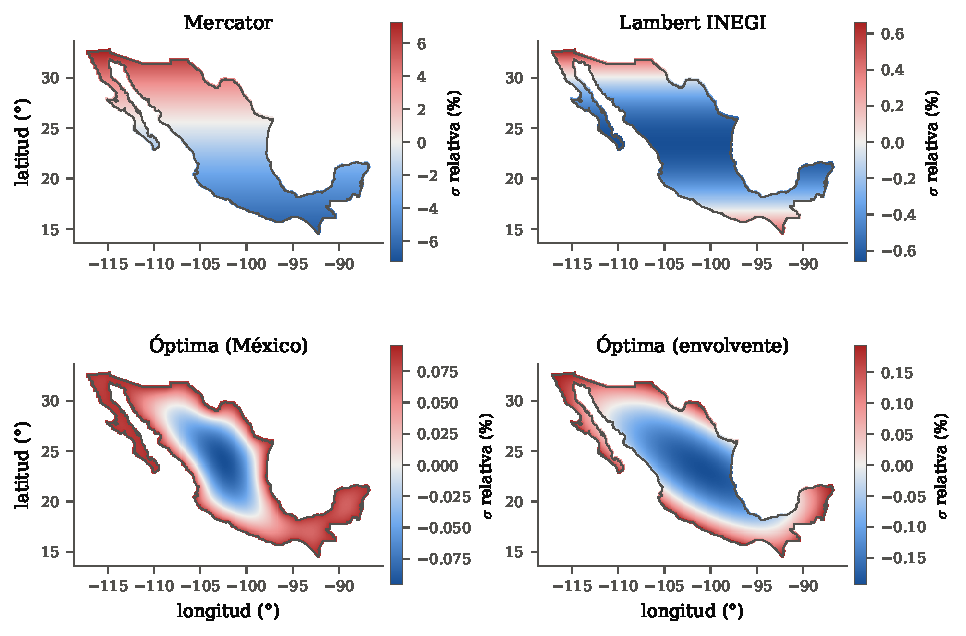
\includegraphics[width=\linewidth]{fig2_sigma}
  \caption{Factor de escala sobre México para cada proyección, reescalado para
    quedar centrado en 1, como desviación en por ciento; la escala de color
    cambia de panel a panel. En la óptima sobre México $\sigma$ es
    prácticamente constante en todo el borde (condición de Chebyshev); en la de
    la envolvente lo es sobre la envolvente convexa. Fuente: elaboración propia.}
  \label{fig:sigma}
\end{figure}

\subsection{Paso 5. Efecto en los datos del cliente}

\paragraph{Datos.} La región $\region$ es México continental, sin islas: la
unión de las 32 entidades del Marco Geoestadístico del INEGI
\cite{inegi_catalogo}, simplificada a 1~km (2061 vértices). Como datos se usan
las cabeceras de los 2478 municipios, tomadas del Catálogo Único de Claves
Geoestadísticas del INEGI (consultado el 26 de noviembre de 2026; en las
alcaldías de la Ciudad de México, la localidad sede). Sin las dos que están en
islas quedan 2476 puntos, que se asignan por entidad a tres regiones: Norte
(BC, BCS, Son., Chih., Coah., NL, Tamps., Dgo., Sin., Zac.; 400 puntos), Sur
(Camp., Chis., Gro., Oax., Q.\,Roo, Tab., Ver., Yuc.; 1136) y Centro (el
resto; 940).

\paragraph{Distancias.} Se tomaron 20\,000 pares al azar dentro de cada región
y 20\,000 en todo el país, y se comparó la distancia euclidiana en cada
proyección con la haversine (figura~\ref{fig:errores}). Con Mercator la mediana
del error es de $5.0\,\%$ en el Sur, $6.3\,\%$ en el Centro y $11.6\,\%$ en el
Norte, con máximos de $18.6\,\%$; corregir con una escala constante no basta,
porque en el Norte la mediana sigue en $5.2\,\%$. Con
Lambert la mediana va de $0.12\,\%$ a $0.41\,\%$ según la región y el máximo
es $0.73\,\%$. Con la óptima la mediana baja a $0.02$--$0.06\,\%$, y en los
pares cuyo arco de círculo máximo queda dentro del territorio (el $88\,\%$ de
la muestra) el error nunca pasa de $0.092\,\%$, que es exactamente la cota
$e^{\delta^*/2} - 1$.

La excepción son los pares que cruzan el mar: entre Baja California Sur y
Sinaloa el error de la óptima llega a $1.8\,\%$, porque la cota solo vale
dentro de $\region$. Resolviendo el problema sobre la envolvente convexa de
México, que incluye los dos golfos, $\delta$ sube a $0.0039$, pero el error
máximo en \emph{todos} los pares de la muestra es de $0.19\,\%$.

\paragraph{Agrupamiento y vecinos.} Se corrió k-means ($k = 10$, $20$ y $50$,
diez semillas) desde los mismos centros que un k-means sobre la esfera y se
contaron los puntos que cambian de grupo (emparejando grupos con el método
húngaro). La mediana de cambios es de $0.7$--$1.5\,\%$ con Mercator,
$0.02$--$0.24\,\%$ con Lambert y $0$--$0.02\,\%$ con la óptima; además, en 7 de
30 corridas con Mercator y en una con Lambert más del $5\,\%$ de los puntos
cambió de grupo porque k-means cayó en otra solución. El conjunto de los 10
vecinos más cercanos cambia en el $0.69\,\%$ de los puntos con Mercator, el
$0.08\,\%$ con Lambert y el $0.12\,\%$ con la óptima (dos cabeceras de Baja
California Sur con vecinos al otro lado del golfo).

\paragraph{Áreas.} Las áreas se multiplican por $\sigma^2$. En las cabeceras,
con Mercator ese factor va de $1.07$ en el Sur a $1.41$ en el Norte, así que un
mapa de densidad subestima la del norte hasta en un $24\,\%$ frente al sur. Con Lambert el
factor está entre $0.989$ y $1.015$, y con la óptima entre $0.998$ y $1.002$.

\begin{figure}[ht]
  \centering
  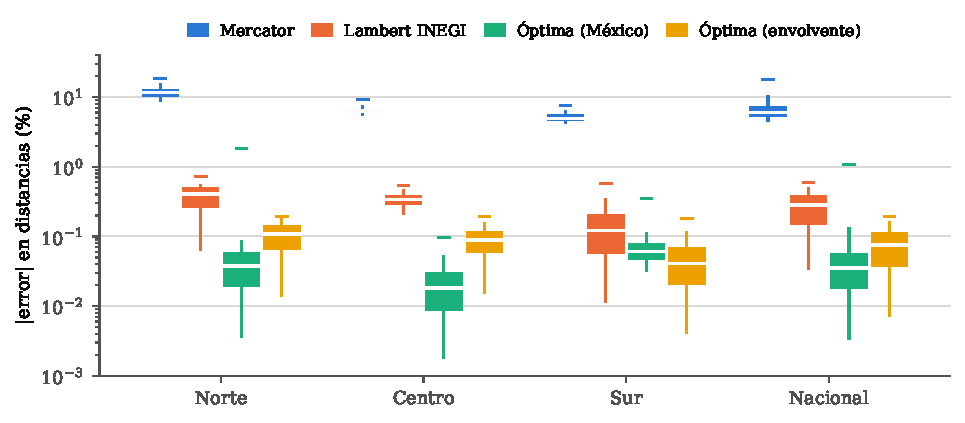
\includegraphics[width=\linewidth]{fig3_errores}
  \caption{Error relativo en distancias entre pares de cabeceras, por región
    y proyección, en escala logarítmica. La caja va del percentil 25 al 75, la
    línea blanca es la mediana, los bigotes van del percentil 5 al 95 y la marca
    aislada es el máximo. Fuente: elaboración propia con datos del INEGI.}
  \label{fig:errores}
\end{figure}

\section{Implementación y verificación}
El contorno simplificado tiene 2061 vértices. Se resuelve $\Delta(h-\ln R)=0$ con borde $\ln\cos\varphi$, mediante diferencias finitas y Shortley--Weller junto a la frontera \cite{shortley1938}. Se usa $\Delta w=0.001$, con 58312 nodos. Las aristas proporcionan incrementos de conjugada y mapa, conciliados por mínimos cuadrados. Un ajuste polinomial previo dejó residuos cercanos a $9\times10^{-4}$, por lo que no se eligió para esta geometría \cite{brubeck2021}.

Con la solución conocida $h=\ln|w-w_*|$, singularidad exterior, los errores máximos son $1.46\times10^{-4}$, $3.74\times10^{-5}$, $9.74\times10^{-6}$ y $2.49\times10^{-6}$ con pasos $0.004$, $0.002$, $0.001$ y $0.0005$: convergencia aproximadamente cuadrática. Las mallas $0.002$, $0.001$ y $0.0005$ dan $\delta=0.00184343$, $0.00184347$ y $0.00184298$. En cabeceras, la prueba a 1 km conserva el ángulo recto a $0.003^\circ$. En los vértices de frontera, la oscilación interpolada de $\ln\sigma$ es $1.11\times10^{-4}$ y la desviación máxima respecto a $c$ es $7.52\times10^{-5}$. Estos residuos reflejan la reconstrucción discreta. La evaluación local puede tener saltos entre celdas de unos 6 mm: se documentan como error numérico, no como propiedad conforme exacta.

Mercator y Lambert esféricas coinciden con PROJ a menos de $10^{-8}$ m \cite{proj}. Los parámetros corresponden a EPSG:6372, \emph{Mexico ITRF2008 / LCC}, no a EPSG:6361, ausente como CRS en la base consultada \cite{epsg}. El código conserva funciones puras para fórmulas y clases para malla y modelo persistente. La carga común evita resolver de nuevo durante cada análisis.

% Responsable: Persona 3. ~100 palabras + tabla.
\section{Herramienta para el cliente}

La tabla~\ref{tab:comparativa} resume las cuatro opciones. Las columnas de
distancias, k-means y vecinos se calcularon con las cabeceras municipales
(Paso~5); k-means corresponde a $k = 20$ (mediana de diez semillas).

\begin{table}[ht]
  \centering
  \footnotesize
  \setlength{\tabcolsep}{4pt}
  \begin{tabular}{lrrrrrrr}
\toprule
 & & Error máx. & \multicolumn{3}{c}{Error en distancias (\%)} & k-means & 10 vecinos \\
\cmidrule(lr){4-6}
Proyección & $\delta$ & escala (\%) & mediana & P95 & máx. & cambios (\%) & cambian (\%) \\
\midrule
Mercator & 0.1402 & 7.26 & 6.07 & 10.21 & 18.04 & 0.67 & 0.69 \\
Lambert INEGI & 0.0132 & 0.66 & 0.28 & 0.49 & 0.60 & 0.24 & 0.08 \\
Óptima (México) & 0.0018 & 0.09 & 0.04 & 0.13 & 1.07 & 0.02 & 0.12 \\
Óptima (envolvente) & 0.0039 & 0.19 & 0.07 & 0.16 & 0.19 & 0.02 & 0.08 \\
\bottomrule
\end{tabular}

  \caption{Comparación de las proyecciones sobre México. El error máximo de
    escala supone el mapa reescalado para centrar $\sigma$ en 1. El máximo de
    la óptima (México) viene de pares que cruzan el Golfo de California.
    Fuente: elaboración propia con datos del INEGI.}
  \label{tab:comparativa}
\end{table}

Para convertir coordenadas, el repositorio incluye la función
\texttt{latlon\_a\_xy(lat, lon, proyeccion="recomendada")} en
\texttt{src/proyecciones/conversion.py}. Recibe grados (números, arreglos o
las columnas de un CSV) y devuelve $x, y$ en metros. La opción recomendada es
la óptima sobre la envolvente convexa, cuyo modelo ya ajustado viene en el
repositorio, así que no hace falta resolver nada; también acepta
\texttt{"optima"}, \texttt{"lambert"} y \texttt{"mercator"}; avisa si un
punto queda fuera de la región, y las filas sin coordenadas quedan vacías. Desde la terminal:
\begin{lstlisting}[basicstyle=\footnotesize\ttfamily]
python -m proyecciones.conversion clientes.csv clientes_xy.csv
\end{lstlisting}
Por ejemplo, con la proyección recomendada la distancia en el plano entre la
Ciudad de México y Monterrey es de 704.78~km, contra 705.93~km sobre la
esfera ($-0.16\,\%$), y entre Monterrey y Mérida, de 1212.99~km contra
1213.52~km ($-0.04\,\%$).

% Responsable: Persona 4. ~200 palabras.
\section{Limitaciones y alcance de validez}

\subsection{Modelo esférico frente al elipsoide}
\subsection{Ángulos sí, áreas no}
\subsection{Límites teóricos}
% Riemann (existencia sin fórmula), Liouville (dim >= 3 solo Möbius).
\subsection{Costo práctico}

% Responsable: Persona 4. ~150 palabras. Cada aplicación con una referencia revisada por pares.
\section{Desarrollos recientes y otras aplicaciones}

Aplanar una superficie curva sin deformar las formas es un problema que
aparece en muchas áreas. En gráficos por computadora, los mapas conformes por
mínimos cuadrados se usan para pegar texturas sobre modelos 3D
\cite{levy2002}, y en neuroimagen la corteza cerebral se lleva de forma
conforme a una esfera o a un plano para comparar cerebros de distintas
personas \cite{gu2004,hurdal2004}. Para superficies dadas como mallas de triángulos
existe una teoría de mapeos conformes discretos: el empaquetamiento de
círculos converge al mapeo de Riemann \cite{rodin1987}, y la equivalencia
conforme de mallas permite aplanarlas con distorsión controlada
\cite{springborn2008}. En física e ingeniería, la transformación de Joukowski
convierte el flujo alrededor de un cilindro en el flujo alrededor de un perfil
alar, y la de Schwarz--Christoffel resuelve problemas de potencial
(electrostática, flujo) en regiones poligonales \cite{driscoll2002}. Los
métodos numéricos también siguen avanzando: los solucionadores
\emph{lightning}, basados en funciones racionales, resuelven la ecuación de
Laplace con muchas cifras correctas y en fracciones de segundo, aun en
regiones con esquinas \cite{gopal2019},
justo el tipo de región que complicó el ajuste polinomial en este trabajo.

\section{Conclusiones y recomendaciones al cliente}
El análisis complejo aporta una construcción: pasa de la métrica esférica a una función analítica, identifica $\ln|f'|$ como potencial armónico y determina su frontera mediante Dirichlet. La comparación demuestra cuánto se gana frente al catálogo: la oscilación de escala baja siete veces respecto a Lambert y 76 respecto a Mercator. Proyectar permite conservar algoritmos planos, aunque no reemplaza toda operación geodésica.

El beneficio termina donde cambian las condiciones del modelo: áreas, recorridos fuera del dominio, exigencia subporcentual frente al elipsoide o distancias comparables con los saltos numéricos. En esos casos se requieren proyecciones equivalentes, una región ampliada o cálculo geodésico directo.

Se recomienda EPSG:6372 como sistema de trabajo interoperable. Con un presupuesto ilustrativo de error de 50 m, su error mediano muestral equivale a esa magnitud cerca de 17 km, y su máximo observado cerca de 7 km. La envolvente desplaza el primer umbral a 33 km, pero no mejora sustancialmente el segundo. Estos umbrales son orientativos, no fronteras universales. Mantener la óptima se justifica si esa reducción típica compensa su costo y el cliente valida sus propios datos.


\bibliographystyle{IEEEtran}
\bibliography{referencias}

\appendix
% Responsables: Persona 2 y Persona 3.
\section{Código}
El código completo está en el repositorio del equipo: \url{https://github.com/...}.


\end{document}
